\PassOptionsToPackage{unicode}{hyperref}
\PassOptionsToPackage{naturalnames}{hyperref}

\documentclass[12pt]{article}

\usepackage[utf8]{inputenc}
\usepackage[T1,T2A]{fontenc}
\usepackage[russian]{babel}
\usepackage{tikz}
\usetikzlibrary{shadows}


\title{Метрика для оценки качества контуров зданий Яндекс.Карт}
\author{Кураленок~И., Кручинин~Д.}

\begin{document}
\maketitle

\section{Постановка задачи}
В связи с развитием технологий распознавания и сегментации изображений, в последнее время решение задачи автоматического построения контуров зданий по спутниковым снимкам выглядит все более реалистичным. Развивать подобные методы невозможно без простой процедуры их оценки. В литературе наиболее популярным методом оценки качества разметки зданий является отношения пересечения и объединения внутренних областей контура (IoU). Данная метрика обладает очевидными преимуществами: она понятна и легко реализуется. С другой стороны использовать ее для практического применения в условиях Яндекс может оказаться нецелесообразно, для чего есть следующие предпосылки:
\begin{itemize}
	\item контуры используются в 3d отображении, где важно количество граней;
	\item в Яндекс устоялось собственное понимание стандартов качества разметки.
\end{itemize}
На данный момент оценка качества контуров зданий в Яндекс осуществляется органолептически сообществом квалифицированных картографов. Целью данной работы является автоматизация этой работы путем разработки метрики попарной близости контуров, которая согласуется с результатами работы картографов. В условиях существования подобной метрики возможно составление репрезентативного множества контуров и канонической разметки к ним, на котором в автоматическом режиме проверять качество альтернативной (автоматической или ручной) разметки.

\section{Предлагаемое решение}
Для построения метрики, предсказывающей экспертные оценки, необходимо измерить зависимость согласованности этой оценки от степени изменения исходных данных. Согласованность экспертов по оригинальным данным является ограничивающим фактором для качества полученной метрики, поэтому ее необходимо исследовать в первую очередь. Еще одним важным компонентом является механизм контролируемого изменения данных, который должен отражать возможные особенности поведения алгоритмов распознавания. Для построения метрики была разработана следующая процедура:
\begin{enumerate}
	\item Зафиксировать набор контуров, характерный для Яндекс.Карт
	\item Провести предварительную оценку качества с целью очистки данных и оценки согласованности экспертов
	\item На очищенных данных провести случайные преобразования контуров
	\item Еще раз оценить экспертами преобразованные контуры
	\item По полученной разметке построить функцию близости контуров, согласующуюся с оценками экспертам
\end{enumerate}
Первая часть работы была возложена на специалистов Яндекс, которые подготовили набор данных используемый для дальнейших шагов. Для экспертной оценки качества разметки был разработан специальный стенд в виде Web-сервиса на основе API Яндекс.Карт в п.~\ref{tool} приводится краткая инструкция по работе с этим инструментом на стороне администратора. Подробности алгоритма преобразования контуров описаны в п.~\ref{morphing}. Общая схема построения метрики и ее реализация описаны в п.~\ref{similarity}. Экспериментальные результаты проделанной работы можно видеть в п.~\ref{experiments}.

\section{Стенд оценки качества контуров}
\label{tool}

\begin{figure*}
\label{tool-screen}
\caption{Вид интерфейса стенда оценки качества контуров}
\begin{center}
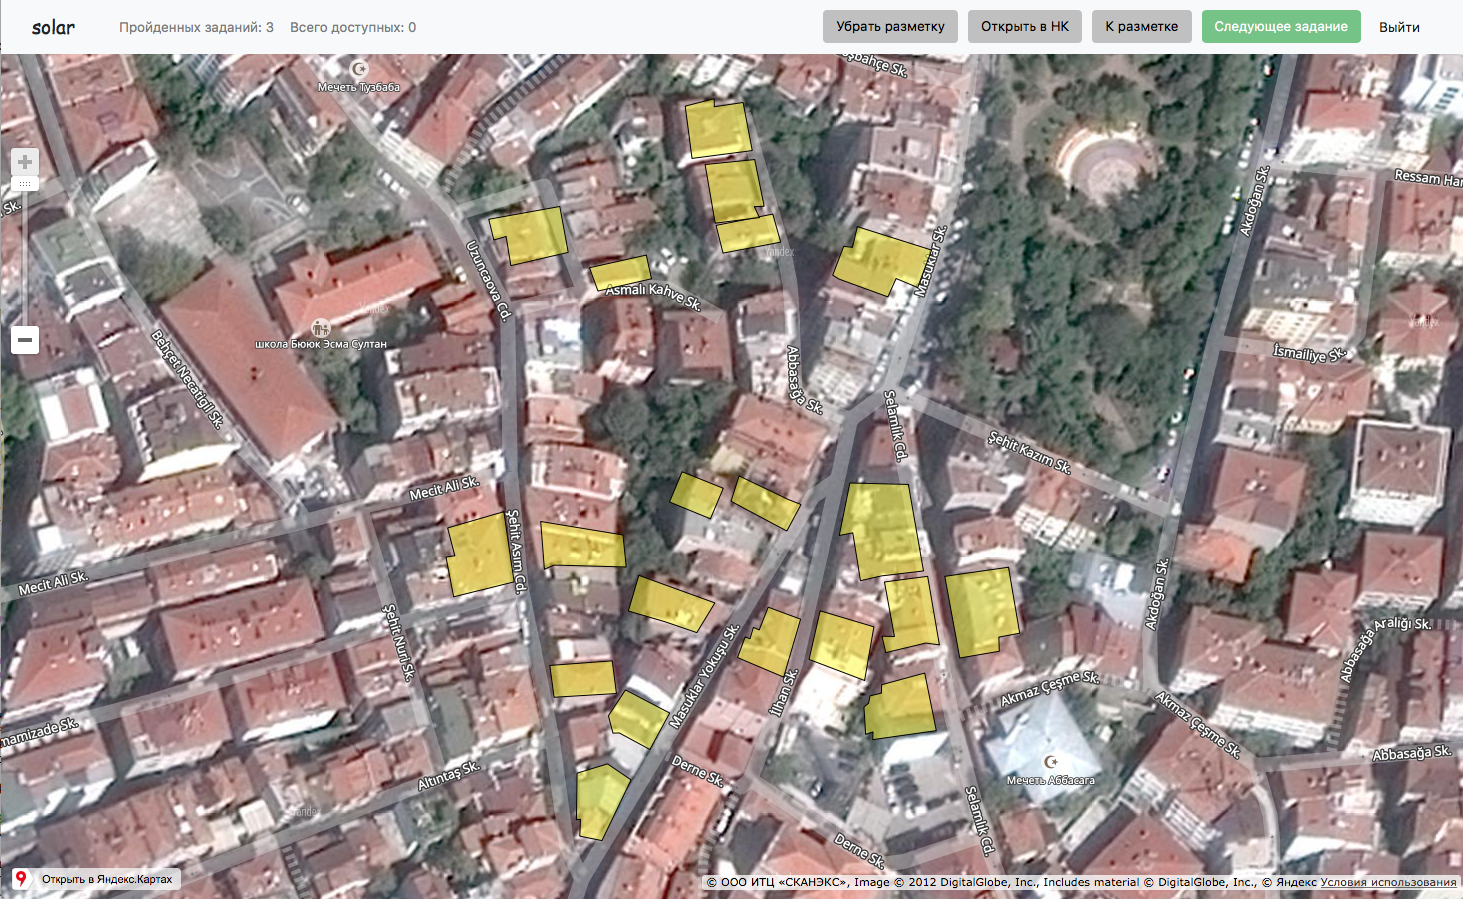
\includegraphics[width=0.75\textwidth]{images/tool-screen-1.png}
\end{center}
\end{figure*}

Для того, чтобы собрать экспертные оценки контуров необходимо создание специализированного инструмента. В качестве платформы для его создания мы выбрали python + flask на серверной стороне и bootstrap + API Яндекс.Карт на клиентской. В результате получился простой инструмент, который может быть использован для экспертной оценки качества произвольных контуров. Выглядит это как на картинке~\ref{tool-screen}.

Пакет для работы стенда находится в директории labeler-app. Далее все примеры приводятся в предположении, что пользователь находится в этой директории.

Для более эффективной работы экспертов контуры сгруппированы в задания по 20 штук (параметр \-\-task\_size), исходя из близости между собой. Чтобы сгенерировать эти задания необходимо воспользоваться утилитой generate\_task.py на вход которой необходимо подать .shp файл. Пример команды генерации заданий:
{\footnotesize
\begin{verbatim}
python3 generate_task.py --data ../sample.shp --out_dir ./data/markup_tasks \
	--task_size 20
\end{verbatim}
}
Труды генератора надо положить в директорию data/markup\_tasks. После изменений заданий необходимо (пере)запустить сервер например такой командой:
{\footnotesize
\begin{verbatim}
nohup python3 server.py & tail -f ./nohup.out
\end{verbatim}
}
После этого сервер стартанет на 5000 порту и на него можно пускать людей. Далее преведена краткая инструкция для экспертов по работе с интерфейсом разметки:

{\footnotesize\begin{verbatim}
Инструмент проверки разметки зданий предназначен для:
 * измерения согласованности разметки экспертами-картографами;
 * выявления зависимости реакции картографа на изменения эталонной разметки;
 * выборочной проверки существующей разметки.

Инструмент выполнен в виде web-приложения, доступного [тут][http://ybmv.expleague.com]

Для начала работы в системе необходимо зарегистрировать нового пользователя. Для
этого необходимо перейти по соответствующей ссылке на стартовой странице. Инфо-
рмацию, введенную при регистрации можно позже использовать для повторного входа в
систему и продолжения работы.

Интерфейс разметки состоит из следующих блоков: карта с оцениваемой разметкой, па-
нель навигации, кнопка перехода к следующему заданию.

Разметка разделена на группы (задания) близких по координатам разметок. По окон-
чанию разметки группы, можно запросить следующую порцию, нажав кнопку «следующее за-
дание».

Для разметки контура, его необходимо выделить с помощью клика по внутренней области.
В появившемся диалоге предлагается принять решение о качестве контура. Если решение
положительное, то внутренняя область будет окрашена в синий цвет, если отрицательное
— в красный. В любой момент до перехода к следующему заданию можно вернуться к уже
размеченному контуру и изменить свое решение.

Для ускорения работы, все действия можно делать с помощью клавиатуры: влево перейдет
к следующему контуру, вправо — к предыдущему, вверх — выделенный контур правильный,
вниз — неверный, Enter перейдет к следующему заданию. Также можно принимать групповые
решения, добавляя к текущему набору контуров другие кликом по ним.
\end{verbatim}}

Результаты работы экспертов синхронно сохраняются на стороне сервера в файле data/results.json. Пример вывода:
{\footnotesize
\begin{verbatim}
[{
    "task": "task140.json",
    "user": "solar",
    "results": [{"id": "2728", "isBad": false}, {"id": "2798", "isBad": false},
    {"id": "1266", "isBad": true},...
\end{verbatim}
}
В приведенном тексте выполнялось задание из файла task140.json в котором были сгруппированы контуры с соотвествтующими id (2728, 2798, etc.) из исходного .shp файла.

\section{Контролируемое ``ухуджение'' контуров}
\label{morphing}
Нам необходимо обеспечить механизм изменения контуров, который мы бы контролировали. Так как контролируемо улучшить результаты разметки мы не можем, поэтому будем ухудшать что делать возможно из-за симметричности отношения. Чтобы отразить особенности поведения алгоритмов распознавания, необходимо учитывать исходное изображение. На первом этапе мы решили этого не делать, а ограничиваться лишь случайными преобразованиями геометрии контура. Данный подход обеспечивает нам оценку снизу для качества распознавания, так как можно предположить скоррелированость ошибок метода и эксперта. Для ухудшения мы использовали групповые и индивидуальные преобразования координат вершин контура. Групповые преобразования, которые мы применяли:
\begin{itemize}
	\item одновременный сдвиг координат контура;
	\item поворот;
	\item масштабирование.
\end{itemize}
Далее каждая вершина случайно сдвигалась на реализацию нормально распределенного случайного вектора. Процесс изменения контура строился следующим образом: координаты контура переводились в метрические, для каждого контура мы бросали случайное количество преобразований ($k \sim Poisson(1)$), далее $k$ раз выбирали из списка равномерно и без повторений преобразование и применяили его. Параметры преобразований фиксировались для каждого контура. Полученные таким образом контуры отправлялись на оценку качества, чтобы по оценке их близости с оригиналом научиться предсказывать оценку эксперта.

\section{Моделирование близости контуров}
\label{similarity}
Для простоты мы рассматривали контуры зданий как двумерные объекты на плоскости и считаем что все вершины контура равнозначны между собой. Для того, чтобы выполнить первое предположение мы предварительно перевели координаты их вершин в метрические. В этом случае преобразование одного контура $X = \{x_i\}$ в другой $Y = \{y_i\}$ можно представить как неточное афинное преобразование:
$$
y_i = A x_i + b + \epsilon
$$
где $A$ и $b$---параметры преобразования, а $\epsilon \sim \mathcal{N}(0, \sigma_0)$---ошибка преобразования. При условии, что контур неособенный и состоит их более чем 3-х точек, подобное преобразование можно восстановить:
\begin{equation}
\label{minimization}
(\hat{A},\hat{b})=\arg \min_{A, b} \frac{1}{|Y|}\sum_i \min_j \|y_i - A x_j + b\|^2_2 + R(A, b)
\end{equation}
и далее использовать параметры и результирующую ошибку $err$ в качестве факторов для оценки близости. В минимизации присутствует загадочный $R(A, b)$, наличие которого обусловленно возможностью нескольких решений, если хотя бы один из контуров центральносимметричен (например квадрат, который можно приляпать ко второму контуру с точностью до поворота). В этом случае $R(A,b)$ позволит выбрать наиболее приемлемую форму решения. Мы используем в качестве регуляризации $R(A, b) = \lambda\left(\|A - E\|_F^2 + \|b\|^2\right)$, где $\lambda$ достаточно мало.

В качестве простейшей модели оценки эксперта $e \in \{-1, 1\}$ можно рассматривать такую:
$$\begin{array}{c}
w = (\hat{A}, \hat{b}, err) \\
P(e = 1| \beta, w) = {e^{\beta^T w} \over 1 + e^{\beta^T w}} = {1 \over 1 + e^{-\beta^T w}}
\end{array}$$
и подобрать ее параметр $\beta$ методом максимального правдоподобия:
$$
\hat{\beta} = \arg \max_\beta \sum_k \log{1 \over 1 + e^{-e_k\beta^T w_k}}
$$
где $e_k$---оценка эксперта $k$-го контура, а $w$---параметры афинного преобразования и его ошибка. Даже такая примитивная модель оказывается неплохо согласуется с поведением экспертов. Однако можно пойти дальше и подобрать более качественную решающую функцию, в частности в виде ансамбля деревьев решений (aka matrixnet :)).

Все шаги приведенной последовательности действий тривиальны за исключением минимизации \ref{minimization}, которая из-за вложенного минимума негладкая. В нашем случае, так как количество точек контура небольшое, можно рассмотреть все варианты соответствия и выбрать наименьший. В этом случае прийдется выполнить $|X|\times|Y|$) 6-ти мерных выпуклых оптимизаций, что для современнных машин несложная задача. Вторым вариантом решения данной задачи является сглаживание целевой функции до формы:
$$
(\hat{A},\hat{b})=\arg \min_{A, b} \frac{1}{|Y|}\sum_{i,j} log(\delta + \|y_i - A x_j + b\|^2_2)
$$
где $\delta >0$---параметр оптимизации.

\section{Использование метрики}
\label{metrica-usage}
Для вычисления метрики можно воспользоваться одной из трех опций: вызов c++ библиотеки, вызов ее порта в python через boost, воспользоваться утилитой из командной строки. Первые 2 варианта проще посмотреть в коде, поэтому остановимся на последнем. Чтобы воспользоваться метрикой необходимо иметь два списка контуров в json формате вида:
{\tiny
\begin{verbatim}
[
[[28.861665402000085, 41.01564292200004], [28.861854402000063, 41.01580092200004], [28.861934975000054, 41.01574611400008]],
[[28.861680767000053, 41.015857001000086], [28.86178576700007, 41.01579200100008], [28.861655504000055, 41.01567272200003]]
]
\end{verbatim}
}
В этих файлах порядок считается идентичным и в результате будет выдана вероятность одинаковой оценки $i$-го контура в первом файле $i$-му во втором. Эти файлы необходимо подать на вход утилите:
{\footnotesize
\begin{verbatim}
ymaprica --real reference.json --gen test.json
\end{verbatim}}
Результатом исполнения этой команды станет колонка чисел от 0 до 1, каждая из которой соответствует значению прогнозируемой вероятности того, что эксперт оценит два контура одинаково.

\section{Результаты эксперимента}
\label{experiments}
Полученные от экспертов данные были разбиты на две части 70\% -- часть для обучения модели и 30\% -- тест. На тестовой выборке посчитаны две метрики качества классификатора: точность и площадь под roc кривой.

Для подсчета точности вероятность $P(e | w)$ переводилась в 1, в случае, если она больше $0.4$ и в 0, в противном случае. Таким образом, результирующая формула -- (кол-во правильно угаданных) / (общее количество семплов). В качестве порога выбрано значение дающее максимальное значение метрики.

Точность классификатора: 0.863\%.

Для того чтобы оценить качество классификатора не подбирая ``порога'', выбрана известная в литературе метрика площадь под roc кривой (ROC AUC). Данная метрика строит кривую из пар значений: (кол-во правильно угаданных позитивов)  / (кол-во позитивов); 1 - (кол-во правильно угаданных негативов) / (кол-во негативов). Разные точки получаются в результате выбора разного порога для $P(e | w)$. Затем считается площадь под этой кривой.

ROC AUC классификатора: 0.886.

Также имеет место интерпретация параметров модели -- $w$. Чем больше модуль числа $w_i$, тем более важен $i$ признак для предсказания. Далее идут значения $w$ для каждого из параметров:
сдвиг по $x$: 0.53780502, сдвиг по $y$: 0.42510037, поворот: 6.64590915, масштаб: 7.68758817, невязка($\delta$) 5.28174901.

\section{Выводы}
\label{conclusions}
В результате работы была построена метрика близости контуров зданий. Данная метрика хорошо согласуется с результатами оценки картографов и может быть использована для первичной оценки качества разметки как автоматических алгоритмов, так и результатов работы полуавтоматических партнерских систем. Было подтверждено, что стандартная метрика IoU существенно хуже подходит для этих целей. В процессе работы над разметкой была выявлена высокая степень согласованности оценок экспертов (около 80\%), что подтверждает обоснованность органолептического подхода к разметке используемого на данный момент в Яндекс.Картах. При разметке данных было выявлено неожианное качество существующей разметки в 70\%, заметим, что это качество существенно зависит от местоположения и в некоторых областях опускается до критически низких значений. Возможно стоит провести детальный анализ этого эффекта.

За рамки этой работы попал вопрос учета фрагментации контура: мы рассматривали попарную близость замкнутых контуров, которая не подходит в ситуации когда возможно разбиение контура на две или более части в связи, например, с разновысотностью фрагментов. Для решения этой задачи может быть использован подход, описанный выше, при условии формализации класса валидных разбиений. Подобную формализацию можно провести на основе сложившейся практики, однако эта задача может быть выполнена только квалифицированным в области картографии коллективом.

В процессе работы был построен стенд оценки качества разметки. На основе подобного подхода возможно построения сравнительной оценки качества Яндекс.Карт с конкурентами. В частности можно получить разметку качества существующих контуров по снимкам конкурентов, чтобы сравнить привязку и качество снимков. Также возможно оценить качество разметки по разным областям на основании близости контуров Яндекс и конкурентов.

\end{document}
